\documentclass[tikz,border=3pt]{standalone}
\usepackage[utf8]{inputenc}
\usepackage[T1]{fontenc}
\usepackage{lmodern}
\renewcommand{\familydefault}{\sfdefault}
\usepackage{sansmath}\sansmath
\usepackage{chemfig}
\usepackage{pgfplots}\pgfplotsset{compat=1.18,/pgf/number format/use comma,/pgf/number format/1000 sep={.}}
\usetikzlibrary{arrows.meta,calc,positioning,decorations.pathmorphing,patterns}
% paleta del sitio
\definecolor{nar}{HTML}{E8680C}\definecolor{narc}{HTML}{FFB35C}\definecolor{hielo}{HTML}{FFF3E8}
\definecolor{tinta}{HTML}{1D1D1F}\definecolor{gris}{HTML}{6E6E73}\definecolor{lila}{HTML}{7C5CF0}
\definecolor{azul}{HTML}{2F6FD6}\definecolor{menta}{HTML}{17A673}\definecolor{coral}{HTML}{E8342A}
\begin{document}
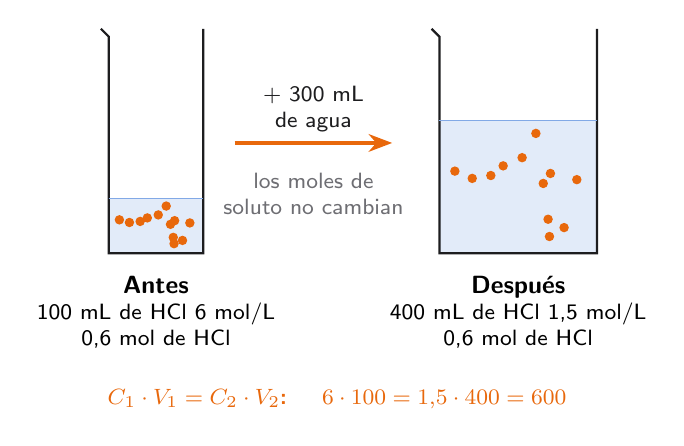
\begin{tikzpicture}[font=\small]
% antes: 100 mL concentrada
\fill[azul!14] (-0.6,0) rectangle (0.6,0.7);
\pgfmathsetseed{8}
\foreach \i in {1,...,12} {\fill[nar] ($(0,0)+(-0.52+1.04*rnd,0.08+0.54*rnd)$) circle (0.06);}
\draw[tinta,thick] (-0.7,2.85) -- (-0.6,2.75) -- (-0.6,0) -- (0.6,0) -- (0.6,2.85);
\draw[azul!60] (-0.6,0.7) -- (0.6,0.7);
\node[align=center,font=\footnotesize] at (0,-0.75) {\textbf{\small Antes}\\100 mL de HCl 6 mol/L\\0,6 mol de HCl};
% agua que se agrega
\draw[-{Stealth[length=3mm]},very thick,nar] (1.0,1.4) -- (3.0,1.4) node[midway,above,tinta,font=\footnotesize,align=center] {+ 300 mL\\de agua};
\node[font=\footnotesize,gris,align=center] at (2.0,0.75) {los moles de\\soluto no cambian};
% despues: 400 mL diluida
\begin{scope}[shift={(4.6,0)}]
\fill[azul!14] (-1.0,0) rectangle (1.0,1.68);
\pgfmathsetseed{8}
\foreach \i in {1,...,12} {\fill[nar] ($(0,0)+(-0.9+1.8*rnd,0.1+1.48*rnd)$) circle (0.06);}
\draw[tinta,thick] (-1.1,2.85) -- (-1.0,2.75) -- (-1.0,0) -- (1.0,0) -- (1.0,2.85);
\draw[azul!60] (-1.0,1.68) -- (1.0,1.68);
\end{scope}
\node[align=center,font=\footnotesize] at (4.6,-0.75) {\textbf{\small Después}\\400 mL de HCl 1,5 mol/L\\0,6 mol de HCl};
\node[font=\footnotesize\bfseries,nar] at (2.3,-1.85) {$C_1 \cdot V_1 = C_2 \cdot V_2$: \quad $6 \cdot 100 = 1{,}5 \cdot 400 = 600$};
\end{tikzpicture}
\end{document}
